\nsection{Dynamic Programming}

% \subsection{Steiner-tree DP}
% \ncomment{$n$ nodes, $k$ terminal nodes, unite all terminal nodes doing a Steiner tree}
% 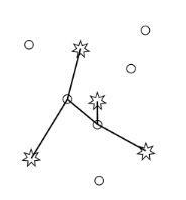
\includegraphics[width = 5cm]{../Codes/DynamicProgramming/SteinerTree.png}
% \addfile{../Codes/DynamicProgramming/Steiner.cpp}
% \vspace{-15pt}

\subsection{All submasks of a mask}
\begin{code}
for (int B = A; B > 0; B = (B - 1) & A)
\end{code}

\subsection{Matrix Chain Multiplication}
\addfile{../Codes/DynamicProgramming/Matrix chain multiplication.cpp}

\subsection{Digit DP} 

\addfile{../Codes/DynamicProgramming/Digit.cpp}

\subsection{Knapsack 0/1}
\addfile[5-7]{../Codes/DynamicProgramming/Knapsack 01.cpp}

\subsection{Convex Hull Trick \complexity{n^2} $\Rightarrow$ \complexity{n}}

\addfile[1-41]{../Codes/DynamicProgramming/Convex hull trick.cpp}

\subsection{Divide and conquer \complexity{kn^2} $\Rightarrow$ \complexity{k \cdot nlogn}} 

\addfile{../Codes/DynamicProgramming/Divide and conquer.cpp}

\subsection{Knuth optimization \complexity{n^3} $\Rightarrow$ \complexity{n^2}} 
$ dp[l][r] = \min_{l \leq k \leq r}\{dp[l][k] + dp[k][r]\} + cost(l, r)$ \\
\addfile[4]{../Codes/DynamicProgramming/Knuth.cpp}